\subsubsection{Principe de la méthode de Debye-Scherrer}

La méthode de Debye-Scherrer est employée pour déterminer la structure cristalline d'un matériau. Elle implique l'orientation d'un faisceau de rayons X monochromatiques vers un échantillon cristallin, induisant ainsi la diffraction des rayons X par les plans du réseau cristallin. En mesurant les angles de diffraction sur le film, il devient possible de calculer les distances interatomiques et de révéler la structure cristalline de l'échantillon. Enfin, une analyse de l'épaisseur des tâches sur le film nous permet d'établir une corrélation entre le diamètre des anneaux observés et la distance intermoléculaire du plan diffractant de différentes espèces chimiques.





\begin{figure}[h!]
	\centering
	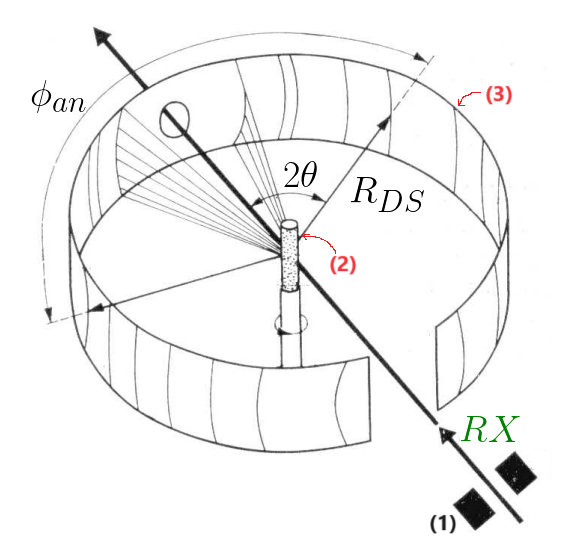
\includegraphics[width=0.7\linewidth]{Méthode_de_Debye_Scherrer/Méthode_de_Debye_Scherrer}
	\caption{\centering Méthode de Debye-Scherrer, (1) : système \{fente + collimateur\}, (2) : poudre de l'élément à analyser , (3) : film , $RX$ : rayon X, $R_{DS}$ : rayon de la chambre de Debye-Scherrer}
	\label{fig:methodededebyescherrer}
\end{figure}
\newpage



\subsubsection{Incertitudes lié à la méthode de Debye-Scherrer}

Cette méthode comporte plusieurs sources d'erreurs. La première provient d'un mauvais centrage de l'échantillon par rapport à l'axe optique du sytème \{fente + collimateur \}, ce qui engendre une incertitude sur l'angle $\theta$.
Pour le calcul de l'incertitude de $\theta$ nous utiliserons les incertitudes de type B (équation \ref{eq: Type B}) appliquer à notre étude (équation \ref{eq:TypeB_theta}):

\begin{equation}\label{eq:TypeB_theta}
	\frac{\Delta \theta}{\theta} = \sqrt{\left ( \frac{\Delta \phi_{an}}{\phi_{an}} \right )^2 + \left ( \frac{\Delta \phi_{DS}}{\phi_{DS}} \right )^2 }
\end{equation}

où :

\begin{itemize}
	\item $\phi_{an}$ : diamètres des anneaux perçu sur le film ;
	
	\item $\Delta A$ : l'incertitude sur la grandeur physique A ;
	

	
	\item $\phi_{DS}$ : diamètre de la chambre de Debye-Scherrer.
	
	\item $\theta = \frac{\phi_{an}}{2\phi_{DS}}$
\end{itemize}

D'après l'énoncé de TP, on a :
\begin{equation}
	\Delta \phi_{an} = \pm 0.5 \ mm  \ / \ \Delta \phi_{DS} = 0.002 \ cm
\end{equation}

On obtient donc le tableau \ref{tab:Tableau des angles correspondant aux diffrentes raies en fonction de phi DS} : 










\begin{table}[h!]
	\centering
	\begin{tabular}{|c|c|c|c|c|}
		
		\hline
Raie	&	$\phi_{an}$ (mm) & $\theta $ (°)	 & $\Delta \theta$ (°) & $\phi_{DS}$ (cm) \\ \hline
1 &	27.4	&           0.238          &    0.02    & 57.35\\ \hline
2 &	31.8	&        0.277              &   0.02     & 57.35\\ \hline
3 &	45.5	&          0.396           &    0.01   & 57.35 \\ \hline
4 &	53.9	&          0.469            &  0.009      & 57.35\\ \hline
 5 &	56.5	&      0.492                 &   0.009   &57.35  \\ \hline
6&	66.3	&            0.492          &     0.008	  & 57.35\\ \hline
7&	74	&               0.645        &     0.007   & 57.35\\ \hline
8&	75.5	&           0.658           &   0.007    & 57.35 \\ \hline
9&	83.8	&            0.730          &   0.006    & 57.35 \\ \hline
	\end{tabular}
	\caption{Angles de diffraction des plans $(h k l)$ avec leurs incertitudes respectives
	 }
	\label{tab:Tableau des angles correspondant aux diffrentes raies en fonction de phi DS}
\end{table}

De même il y aura une incertitude sur $d_{hkl}$ on la calcul donc en appliquant l'équation \ref{eq: Type B} :

\begin{equation} \label{eq: Type B dhkl}
	\frac{\Delta d_{hkl}}{d_{hkl}} = \sqrt{\left ( \frac{\Delta \lambda }{\lambda} \right )^2 + \left ( \frac{\Delta \theta}{\tan(\theta)} \right )^2 }
\end{equation}

De plus, d'après l'énoncé de TP, on a		  :

\begin{equation}
	\lambda = 1.539 \AA \ / \ \Delta \lambda = 0.001 \AA
\end{equation}

\newpage
Cela nous permet d'avoir le tableau \ref{tab:Tableau des dhkl correspondant aux différentes raies}
\begin{table}[h!]
	\centering
	\begin{tabular}{|c|c|c|}
		
		\hline
	Raie &	$ d_{hkl} (\AA) $& $\Delta d_{hkl} (\AA)$  \\ \hline
	 1& 3.252	&         0.02                     \\ \hline
	2& 2.811	&      0.02                         \\ \hline
	3& 1.992	&       0.01                       \\ \hline
	4& 1.699	&         0.009                     \\ \hline
	5& 1.627	&        0.008                       \\ \hline
	6&1.408	&          0.007                     \\ \hline
	7& 1.280	&       0.006                        \\ \hline
	8& 1.258	&       0.006                        \\ \hline
	9& 1.153	&        0.005                       \\ \hline
	\end{tabular}
	\caption{Distances interréticulaires des plans $(h k l)$ avec leurs incertitudes respectives}
	\label{tab:Tableau des dhkl correspondant aux différentes raies}
\end{table}

D'après l'énoncé de TP, nous avons une forte intensité lumineuse pour les raies $(2, 3, 5)$. Par conséquent, en se référant au tableau \ref{tab:Tableau des dhkl correspondant aux différentes raies}, nous avons les valeurs suivantes :

\begin{equation}
	d_1 = 2.811 \ \text{Å} \pm 0.02 \ \text{Å}, \quad d_2 = 1.992 \ \text{Å} \pm 0.01 \ \text{Å}, \quad d_5 = 1.627 \ \text{Å} \pm 0.008 \ \text{Å}
\end{equation}

Ces valeurs de $(d_1, d_2, d_5)$ correspondent aux valeurs lié au NaCl donné par le Handbook, donc nous avons\textbf{ présence de NaCl dans la poudre}.

\subsubsection{Détermination du réseau}

\begin{flushleft}
	On sait, d'après l'énoncé de  TP, que la maille de l'élément étudié est cubique. Notre objectif est alors de déterminer si cette maille présente une structure cubique faces centrées (CFC) ou une structure cubique centrée (CC).
	
	
	Dans le cas d’une maille (CFC), les indices de Miller $(h k l)$ doivent vérifier la condition
	suivante afin que l’on observe le phénomène de diffraction : 
	\begin{center} 
		$\forall (h,k,l)\in \mathbb{Z}^3,$  $h,k,l$ ont la même parité 
	\end{center}
	
	pour une  maille (CC) les indices de Miller $(h k l)$ doivent vérifier la condition : 
	
	\begin{equation}
		\forall (h,k,l)\in \mathbb{Z}^3, \ 	h + k + l = 2n, \ n \in \mathbb{N}
	\end{equation}


\newpage
Le tableau \ref{tab:Listes des plans diffractants pour la structure (CC) et (CFC) (marqué d’un "OK")} répertorie les neuf premiers plans diffractants pour la structure (CC) et (CFC).
\begin{table}[h!]
	\centering
	\begin{tabular}{|c|c|c|c|}
		\hline
		\textbf{Indice plans $(h k l)$} & \textbf{$N=h^2+k^2+l^2$} & \textbf{(CC)} & \textbf{(CFC)} \\
		\hline
		1 0 0 & 1 & 0 & 0 \\
		\hline
		1 1 0 & 2 & \textcolor{myred}{OK }& 0 \\
		\hline
		1 1 1 & 3 & 0 & \textcolor{myred}{OK } \\
		\hline
		2 0 0 & 4 & \textcolor{myred}{OK } & \textcolor{myred}{OK } \\
		\hline
		2 1 0 & 5 & 0 & 0 \\
		\hline
		2 1 1 & 6 & \textcolor{myred}{OK } & 0 \\
		\hline
		2 2 0 & 8 & \textcolor{myred}{OK } & \textcolor{myred}{OK } \\
		\hline
		3 0 0 & 9 & 0 & 0 \\
		\hline
		3 1 0 & 10 & \textcolor{myred}{OK } & 0 \\
		\hline
		3 1 1 & 11 & 0 & \textcolor{myred}{OK } \\
		\hline
		2 2 2 & 12 & \textcolor{myred}{OK } & \textcolor{myred}{OK } \\
		\hline
	\end{tabular}
	\caption{Listes des plans diffractants pour la structure (CC) et (CFC) (marqué d’un \textcolor{myred}{OK})}
	\label{tab:Listes des plans diffractants pour la structure (CC) et (CFC) marqué d’un "OK"}
\end{table}


Le tableau \ref{tab:Comparaison des rapport des distances inter-réticulaires d1/d2, d2/d3 et d1/d3 pour la poudre à celle du Handbook} est construit afin de comparer les distances interréticulaires
	d1/d2, d2/d3 et d1/d3 pour la poudre, pour les deux mailles (CC) et (CFC).

\begin{table}[h!]
	\centering
	\begin{tabular}{|c|c|c|}
		\hline
		 Rapport $d_{hkl}$ (CC)  &  Rapport $d_{hkl}$ (CFC) &  Données du Handbook (NaCl)\\
		\hline
		 $\frac{d_{200}}{d_{211}} = 1.225 $ & $\frac{d_{200}}{d_{220}} = 1.414 $  & $\frac{d_{1}}{d_{2}} = 1.417 $  \\
		\hline
		 $\frac{d_{211}}{d_{310}} = 1.291 $ & $\frac{d_{220}}{d_{222}} = 1.224 $  & $\frac{d_{2}}{d_{3}} = 1.221 $  \\
		\hline
		 $\frac{d_{200}}{d_{310}} = 1.581 $ & $\frac{d_{200}}{d_{222}} = 1.732 $  & $\frac{d_{1}}{d_{3}} = 1.730 $ \\
		\hline
	\end{tabular}
	\caption{\centering Comparaison des rapport des distances inter-réticulaires d1/d2, d2/d3 et d1/d3 pour la poudre à celle du Handbook}
	\label{tab:Comparaison des rapport des distances inter-réticulaires d1/d2, d2/d3 et d1/d3 pour la poudre à celle du Handbook}
\end{table}




	Après analyse du tableau \ref{tab:Comparaison des rapport des distances inter-réticulaires d1/d2, d2/d3 et d1/d3 pour la poudre à celle du Handbook}  nous remarquons qu'il y a forte correspandance avec la \textbf{maille (CFC)}. 
	
	

\end{flushleft}


\subsubsection{Paramètre de maille}
\begin{flushleft}
	On a par définition :
	
	\begin{equation}
		d_{hkl} = \frac{1}{\left\| \vec{r^*}_{hkl}^{}  \right\|} , \vec{r^*}_{hkl} = h\vec{a^*} + k\vec{b^*} + l\vec{c^*}
	\end{equation}
	
	où : $(\vec{a^*},\vec{b^*},\vec{c^*})$ est la base du réseau réciproque de la maille étudier.
	
	Or, pour une structure CFC, on a : 
	
	\begin{equation}\label{eq: d_hkl CFC}
		d_{hkl} = \frac{a}{\sqrt{h^2+ k^2 +l^2 }}
	\end{equation} 
	
	où : $a$ est le paramètre de maille du cristal étudier.


\vspace{0.2cm}
	En prenant le deuxième anneau, on obtient :
	
\begin{equation} \label{eq: anneau}
	d_2 = d_{200} = 2,82 \, \text{\AA}
\end{equation}	

De l'équation \ref{eq: anneau} et \ref{eq: d_hkl CFC} on en déduit donc :
\begin{equation}
		 a = \sqrt{2}d_{200}  = 5.64 \, \text{\AA}
\end{equation}


	
	Du fait qu'il n'y a pas d'erreur sur $N$, on a :
	\begin{equation}
			 \Delta a = \frac{\Delta d}{d}
	\end{equation}

	
Or	d'après le tableau \ref{tab:Tableau des dhkl correspondant aux différentes raies} : 
	
	\begin{equation}
		\Delta d_{200} = 0.02 \, \text{\AA} 
	\end{equation} 
	
Finalement, le paramètre de maille du réseau cubique face centrée de la poudre NaCl est :

\begin{equation}
 \boxed{a = 5.64 \AA \pm 0.1 \, \text{\AA}}	
\end{equation} 
	
\end{flushleft}
